%%%%%%%%%%%%%%%%%%%%%%%%%%%%%%%%%%%%%%%%%
%  My documentation report
%  Objetive: Explain what I did and how, so someone can continue with the investigation
%
% Important note:
% Chapter heading images should have a 2:1 width:height ratio,
% e.g. 920px width and 460px height.
%
%%%%%%%%%%%%%%%%%%%%%%%%%%%%%%%%%%%%%%%%%

%----------------------------------------------------------------------------------------
%	PACKAGES AND OTHER DOCUMENT CONFIGURATIONS
%----------------------------------------------------------------------------------------

\documentclass[11pt,fleqn]{book} % Default font size and left-justified equations

\usepackage[top=3cm,bottom=3cm,left=3.2cm,right=3.2cm,headsep=10pt,letterpaper]{geometry} % Page margins
\usepackage{graphicx}
\usepackage{xcolor} % Required for specifying colors by name
\definecolor{darkgreen}{RGB}{0, 153, 0} % Define the orange color used for highlighting throughout the book

% Font Settings
\usepackage{avant} % Use the Avantgarde font for headings
%\usepackage{times} % Use the Times font for headings
\usepackage{mathptmx} % Use the Adobe Times Roman as the default text font together with math symbols from the Sym­bol, Chancery and Com­puter Modern fonts

\usepackage{microtype} % Slightly tweak font spacing for aesthetics
\usepackage[utf8]{inputenc} % Required for including letters with accents
\usepackage[T1]{fontenc} % Use 8-bit encoding that has 256 glyphs

% Bibliography
\usepackage[style=alphabetic,sorting=nyt,sortcites=true,autopunct=true,babel=hyphen,hyperref=true,abbreviate=false,backref=true,backend=biber]{biblatex}
\addbibresource{bibliography.bib} % BibTeX bibliography file
\defbibheading{bibempty}{}

%----------------------------------------------------------------------------------------
%	VARIOUS REQUIRED PACKAGES
%----------------------------------------------------------------------------------------

\usepackage{titlesec} % Allows customization of titles

\usepackage{graphicx} % Required for including pictures
\graphicspath{{Pictures/}} % Specifies the directory where pictures are stored

\usepackage{lipsum} % Inserts dummy text

\usepackage{tikz} % Required for drawing custom shapes

\usepackage[english]{babel} % English language/hyphenation

\usepackage{enumitem} % Customize lists
\setlist{nolistsep} % Reduce spacing between bullet points and numbered lists

\usepackage{booktabs} % Required for nicer horizontal rules in tables

\usepackage{eso-pic} % Required for specifying an image background in the title page

%----------------------------------------------------------------------------------------
%	MAIN TABLE OF CONTENTS
%----------------------------------------------------------------------------------------

\usepackage{titletoc} % Required for manipulating the table of contents

\contentsmargin{0cm} % Removes the default margin
% Chapter text styling
\titlecontents{chapter}[1.25cm] % Indentation
{\addvspace{15pt}\large\sffamily\bfseries} % Spacing and font options for chapters
{\color{darkgreen!60}\contentslabel[\Large\thecontentslabel]{1.25cm}\color{darkgreen}} % Chapter number
{}  
{\color{darkgreen!60}\normalsize\sffamily\bfseries\;\titlerule*[.5pc]{.}\;\thecontentspage} % Page number
% Section text styling
\titlecontents{section}[1.25cm] % Indentation
{\addvspace{5pt}\sffamily\bfseries} % Spacing and font options for sections
{\contentslabel[\thecontentslabel]{1.25cm}} % Section number
{}
{\sffamily\hfill\color{black}\thecontentspage} % Page number
[]
% Subsection text styling
\titlecontents{subsection}[1.25cm] % Indentation
{\addvspace{1pt}\sffamily\small} % Spacing and font options for subsections
{\contentslabel[\thecontentslabel]{1.25cm}} % Subsection number
{}
{\sffamily\;\titlerule*[.5pc]{.}\;\thecontentspage} % Page number
[] 

%----------------------------------------------------------------------------------------
%	MINI TABLE OF CONTENTS IN CHAPTER HEADS
%----------------------------------------------------------------------------------------

% Section text styling
\titlecontents{lsection}[0em] % Indendating
{\footnotesize\sffamily} % Font settings
{}
{}
{}

% Subsection text styling
\titlecontents{lsubsection}[.5em] % Indentation
{\normalfont\footnotesize\sffamily} % Font settings
{}
{}
{}
 
%----------------------------------------------------------------------------------------
%	PAGE HEADERS
%----------------------------------------------------------------------------------------

\usepackage{fancyhdr} % Required for header and footer configuration

\pagestyle{fancy}
\renewcommand{\chaptermark}[1]{\markboth{\sffamily\normalsize\bfseries\chaptername\ \thechapter.\ #1}{}} % Chapter text font settings
\renewcommand{\sectionmark}[1]{\markright{\sffamily\normalsize\thesection\hspace{5pt}#1}{}} % Section text font settings
\fancyhf{} \fancyhead[LE,RO]{\sffamily\normalsize\thepage} % Font setting for the page number in the header
\fancyhead[LO]{\rightmark} % Print the nearest section name on the left side of odd pages
\fancyhead[RE]{\leftmark} % Print the current chapter name on the right side of even pages
\renewcommand{\headrulewidth}{0.5pt} % Width of the rule under the header
\addtolength{\headheight}{2.5pt} % Increase the spacing around the header slightly
\renewcommand{\footrulewidth}{0pt} % Removes the rule in the footer
\fancypagestyle{plain}{\fancyhead{}\renewcommand{\headrulewidth}{0pt}} % Style for when a plain pagestyle is specified

% Removes the header from odd empty pages at the end of chapters
\makeatletter
\renewcommand{\cleardoublepage}{
\clearpage\ifodd\c@page\else
\hbox{}
\vspace*{\fill}
\thispagestyle{empty}
\newpage
\fi}

%----------------------------------------------------------------------------------------
%	THEOREM STYLES
%----------------------------------------------------------------------------------------

\usepackage{amsmath,amsfonts,amssymb,amsthm} % For math equations, theorems, symbols, etc

\newcommand{\intoo}[2]{\mathopen{]}#1\,;#2\mathclose{[}}
\newcommand{\ud}{\mathop{\mathrm{{}d}}\mathopen{}}
\newcommand{\intff}[2]{\mathopen{[}#1\,;#2\mathclose{]}}
\newtheorem{notation}{Notation}[chapter]

%%%%%%%%%%%%%%%%%%%%%%%%%%%%%%%%%%%%%%%%%%%%%%%%%%%%%%%%%%%%%%%%%%%%%%%%%%%
%%%%%%%%%%%%%%%%%%%% dedicated to boxed/framed environements %%%%%%%%%%%%%%
%%%%%%%%%%%%%%%%%%%%%%%%%%%%%%%%%%%%%%%%%%%%%%%%%%%%%%%%%%%%%%%%%%%%%%%%%%%
\newtheoremstyle{ocrenumbox}% % Theorem style name
{0pt}% Space above
{0pt}% Space below
{\normalfont}% % Body font
{}% Indent amount
{\small\bf\sffamily\color{darkgreen}}% % Theorem head font
{\;}% Punctuation after theorem head
{0.25em}% Space after theorem head
{\small\sffamily\color{darkgreen}\thmname{#1}\nobreakspace\thmnumber{\@ifnotempty{#1}{}\@upn{#2}}% Theorem text (e.g. Theorem 2.1)
\thmnote{\nobreakspace\the\thm@notefont\sffamily\bfseries\color{black}---\nobreakspace#3.}} % Optional theorem note
\renewcommand{\qedsymbol}{$\blacksquare$}% Optional qed square

\newtheoremstyle{blacknumex}% Theorem style name
{5pt}% Space above
{5pt}% Space below
{\normalfont}% Body font
{} % Indent amount
{\small\bf\sffamily}% Theorem head font
{\;}% Punctuation after theorem head
{0.25em}% Space after theorem head
{\small\sffamily{\tiny\ensuremath{\blacksquare}}\nobreakspace\thmname{#1}\nobreakspace\thmnumber{\@ifnotempty{#1}{}\@upn{#2}}% Theorem text (e.g. Theorem 2.1)
\thmnote{\nobreakspace\the\thm@notefont\sffamily\bfseries---\nobreakspace#3.}}% Optional theorem note

\newtheoremstyle{blacknumbox} % Theorem style name
{0pt}% Space above
{0pt}% Space below
{\normalfont}% Body font
{}% Indent amount
{\small\bf\sffamily}% Theorem head font
{\;}% Punctuation after theorem head
{0.25em}% Space after theorem head
{\small\sffamily\thmname{#1}\nobreakspace\thmnumber{\@ifnotempty{#1}{}\@upn{#2}}% Theorem text (e.g. Theorem 2.1)
\thmnote{\nobreakspace\the\thm@notefont\sffamily\bfseries---\nobreakspace#3.}}% Optional theorem note

%%%%%%%%%%%%%%%%%%%%%%%%%%%%%%%%%%%%%%%%%%%%%%%%%%%%%%%%%%%%%%%%%%%%%%%%%%%
%%%%%%%%%%%%% dedicated to non-boxed/non-framed environements %%%%%%%%%%%%%
%%%%%%%%%%%%%%%%%%%%%%%%%%%%%%%%%%%%%%%%%%%%%%%%%%%%%%%%%%%%%%%%%%%%%%%%%%%
\newtheoremstyle{ocrenum}% % Theorem style name
{5pt}% Space above
{5pt}% Space below
{\normalfont}% % Body font
{}% Indent amount
{\small\bf\sffamily\color{darkgreen}}% % Theorem head font
{\;}% Punctuation after theorem head
{0.25em}% Space after theorem head
{\small\sffamily\color{darkgreen}\thmname{#1}\nobreakspace\thmnumber{\@ifnotempty{#1}{}\@upn{#2}}% Theorem text (e.g. Theorem 2.1)
\thmnote{\nobreakspace\the\thm@notefont\sffamily\bfseries\color{black}---\nobreakspace#3.}} % Optional theorem note
\renewcommand{\qedsymbol}{$\blacksquare$}% Optional qed square
\makeatother

% Defines the theorem text style for each type of theorem to one of the three styles above
\newcounter{dummy} 
\numberwithin{dummy}{section}
\theoremstyle{ocrenumbox}
\newtheorem{theoremeT}[dummy]{Theorem}
\newtheorem{problem}{Problem}[chapter]
\newtheorem{exerciseT}{Exercise}[chapter]
\theoremstyle{blacknumex}
\newtheorem{exampleT}{Example}[chapter]
\theoremstyle{blacknumbox}
\newtheorem{vocabulary}{Vocabulary}[chapter]
\newtheorem{definitionT}{Definition}[section]
\newtheorem{corollaryT}[dummy]{Corollary}
\theoremstyle{ocrenum}
\newtheorem{proposition}[dummy]{Proposition}

%----------------------------------------------------------------------------------------
%	DEFINITION OF COLORED BOXES
%----------------------------------------------------------------------------------------

\RequirePackage[framemethod=default]{mdframed} % Required for creating the theorem, definition, exercise and corollary boxes

% Theorem box
\newmdenv[skipabove=7pt,
skipbelow=7pt,
backgroundcolor=black!5,
linecolor=darkgreen,
innerleftmargin=5pt,
innerrightmargin=5pt,
innertopmargin=5pt,
leftmargin=0cm,
rightmargin=0cm,
innerbottommargin=5pt]{tBox}

% Exercise box	  
\newmdenv[skipabove=7pt,
skipbelow=7pt,
rightline=false,
leftline=true,
topline=false,
bottomline=false,
backgroundcolor=darkgreen!10,
linecolor=darkgreen,
innerleftmargin=5pt,
innerrightmargin=5pt,
innertopmargin=5pt,
innerbottommargin=5pt,
leftmargin=0cm,
rightmargin=0cm,
linewidth=4pt]{eBox}	

% Definition box
\newmdenv[skipabove=7pt,
skipbelow=7pt,
rightline=false,
leftline=true,
topline=false,
bottomline=false,
linecolor=darkgreen,
innerleftmargin=5pt,
innerrightmargin=5pt,
innertopmargin=0pt,
leftmargin=0cm,
rightmargin=0cm,
linewidth=4pt,
innerbottommargin=0pt]{dBox}	

% Corollary box
\newmdenv[skipabove=7pt,
skipbelow=7pt,
rightline=false,
leftline=true,
topline=false,
bottomline=false,
linecolor=gray,
backgroundcolor=black!5,
innerleftmargin=5pt,
innerrightmargin=5pt,
innertopmargin=5pt,
leftmargin=0cm,
rightmargin=0cm,
linewidth=4pt,
innerbottommargin=5pt]{cBox}

% Creates an environment for each type of theorem and assigns it a theorem text style from the "Theorem Styles" section above and a colored box from above
\newenvironment{theorem}{\begin{tBox}\begin{theoremeT}}{\end{theoremeT}\end{tBox}}
\newenvironment{exercise}{\begin{eBox}\begin{exerciseT}}{\hfill{\color{darkgreen}\tiny\ensuremath{\blacksquare}}\end{exerciseT}\end{eBox}}				  
\newenvironment{definition}{\begin{dBox}\begin{definitionT}}{\end{definitionT}\end{dBox}}	
\newenvironment{example}{\begin{exampleT}}{\hfill{\tiny\ensuremath{\blacksquare}}\end{exampleT}}		
\newenvironment{corollary}{\begin{cBox}\begin{corollaryT}}{\end{corollaryT}\end{cBox}}	

%----------------------------------------------------------------------------------------
%	REMARK ENVIRONMENT
%----------------------------------------------------------------------------------------

\newenvironment{remark}{\par\vspace{10pt}\small % Vertical white space above the remark and smaller font size
\begin{list}{}{
\leftmargin=35pt % Indentation on the left
\rightmargin=25pt}\item\ignorespaces % Indentation on the right
\makebox[-2.5pt]{\begin{tikzpicture}[overlay]
\node[draw=darkgreen!60,line width=1pt,circle,fill=darkgreen!25,font=\sffamily\bfseries,inner sep=2pt,outer sep=0pt] at (-15pt,0pt){\textcolor{darkgreen}{R}};\end{tikzpicture}} % Orange R in a circle
\advance\baselineskip -1pt}{\end{list}\vskip5pt} % Tighter line spacing and white space after remark

%----------------------------------------------------------------------------------------
%	SECTION NUMBERING IN THE MARGIN
%----------------------------------------------------------------------------------------

\makeatletter
\renewcommand{\@seccntformat}[1]{\llap{\textcolor{darkgreen}{\csname the#1\endcsname}\hspace{1em}}}                    
\renewcommand{\section}{\@startsection{section}{1}{\z@}
{-4ex \@plus -1ex \@minus -.4ex}
{1ex \@plus.2ex }
{\normalfont\large\sffamily\bfseries}}
\renewcommand{\subsection}{\@startsection {subsection}{2}{\z@}
{-3ex \@plus -0.1ex \@minus -.4ex}
{0.5ex \@plus.2ex }
{\normalfont\sffamily\bfseries}}
\renewcommand{\subsubsection}{\@startsection {subsubsection}{3}{\z@}
{-2ex \@plus -0.1ex \@minus -.2ex}
{.2ex \@plus.2ex }
{\normalfont\small\sffamily\bfseries}}                        
\renewcommand\paragraph{\@startsection{paragraph}{4}{\z@}
{-2ex \@plus-.2ex \@minus .2ex}
{.1ex}
{\normalfont\small\sffamily\bfseries}}

%----------------------------------------------------------------------------------------
%	HYPERLINKS IN THE DOCUMENTS
%----------------------------------------------------------------------------------------

% For an unclear reason, the package should be loaded now and not later
\usepackage{hyperref}
\hypersetup{hidelinks,backref=true,pagebackref=true,hyperindex=true,colorlinks=false,breaklinks=true,urlcolor= darkgreen,bookmarks=true,bookmarksopen=false,pdftitle={Title},pdfauthor={Author}}

%----------------------------------------------------------------------------------------
%	CHAPTER HEADINGS
%----------------------------------------------------------------------------------------

% The set-up below should be (sadly) manually adapted to the overall margin page septup controlled by the geometry package loaded in the main.tex document. It is possible to implement below the dimensions used in the goemetry package (top,bottom,left,right)... TO BE DONE

\newcommand{\thechapterimage}{}
\newcommand{\chapterimage}[1]{\renewcommand{\thechapterimage}{#1}}

% Numbered chapters with mini tableofcontents
\def\thechapter{\arabic{chapter}}
\def\@makechapterhead#1{
\thispagestyle{empty}
{\centering \normalfont\sffamily
\ifnum \c@secnumdepth >\m@ne
\if@mainmatter
\startcontents
\begin{tikzpicture}[remember picture,overlay]
\node at (current page.north west)
{\begin{tikzpicture}[remember picture,overlay]
\node[anchor=north west,inner sep=0pt] at (0,0) {\includegraphics[width=\paperwidth]{\thechapterimage}};
%%%%%%%%%%%%%%%%%%%%%%%%%%%%%%%%%%%%%%%%%%%%%%%%%%%%%%%%%%%%%%%%%%%%%%%%%%%%%%%%%%%%%
% Commenting the 3 lines below removes the small contents box in the chapter heading
%\fill[color=darkgreen!10!white,opacity=.6] (1cm,0) rectangle (8cm,-7cm);
%\node[anchor=north west] at (1.1cm,.35cm) {\parbox[t][8cm][t]{6.5cm}{\huge\bfseries\flushleft \printcontents{l}{1}{\setcounter{tocdepth}{2}}}};
\draw[anchor=west] (5cm,-9cm) node [rounded corners=20pt,fill=darkgreen!10!white,text opacity=1,draw=darkgreen,draw opacity=1,line width=1.5pt,fill opacity=.6,inner sep=12pt]{\huge\sffamily\bfseries\textcolor{black}{\thechapter. #1\strut\makebox[22cm]{}}};
%%%%%%%%%%%%%%%%%%%%%%%%%%%%%%%%%%%%%%%%%%%%%%%%%%%%%%%%%%%%%%%%%%%%%%%%%%%%%%%%%%%%%
\end{tikzpicture}};
\end{tikzpicture}}
\par\vspace*{230\p@}
\fi
\fi}

% Unnumbered chapters without mini tableofcontents (could be added though) 
\def\@makeschapterhead#1{
\thispagestyle{empty}
{\centering \normalfont\sffamily
\ifnum \c@secnumdepth >\m@ne
\if@mainmatter
\begin{tikzpicture}[remember picture,overlay]
\node at (current page.north west)
{\begin{tikzpicture}[remember picture,overlay]
\node[anchor=north west,inner sep=0pt] at (0,0) {\includegraphics[width=\paperwidth]{\thechapterimage}};
\draw[anchor=west] (5cm,-9cm) node [rounded corners=20pt,fill=darkgreen!10!white,fill opacity=.6,inner sep=12pt,text opacity=1,draw=darkgreen,draw opacity=1,line width=1.5pt]{\huge\sffamily\bfseries\textcolor{black}{#1\strut\makebox[22cm]{}}};
\end{tikzpicture}};
\end{tikzpicture}}
\par\vspace*{230\p@}
\fi
\fi
}
\makeatother % Insert the commands.tex file which contains the majority of the structure behind the template

\begin{document}

%----------------------------------------------------------------------------------------
%	TITLE PAGE
%----------------------------------------------------------------------------------------

\begingroup
\thispagestyle{empty}
\AddToShipoutPicture*{\put(0,0){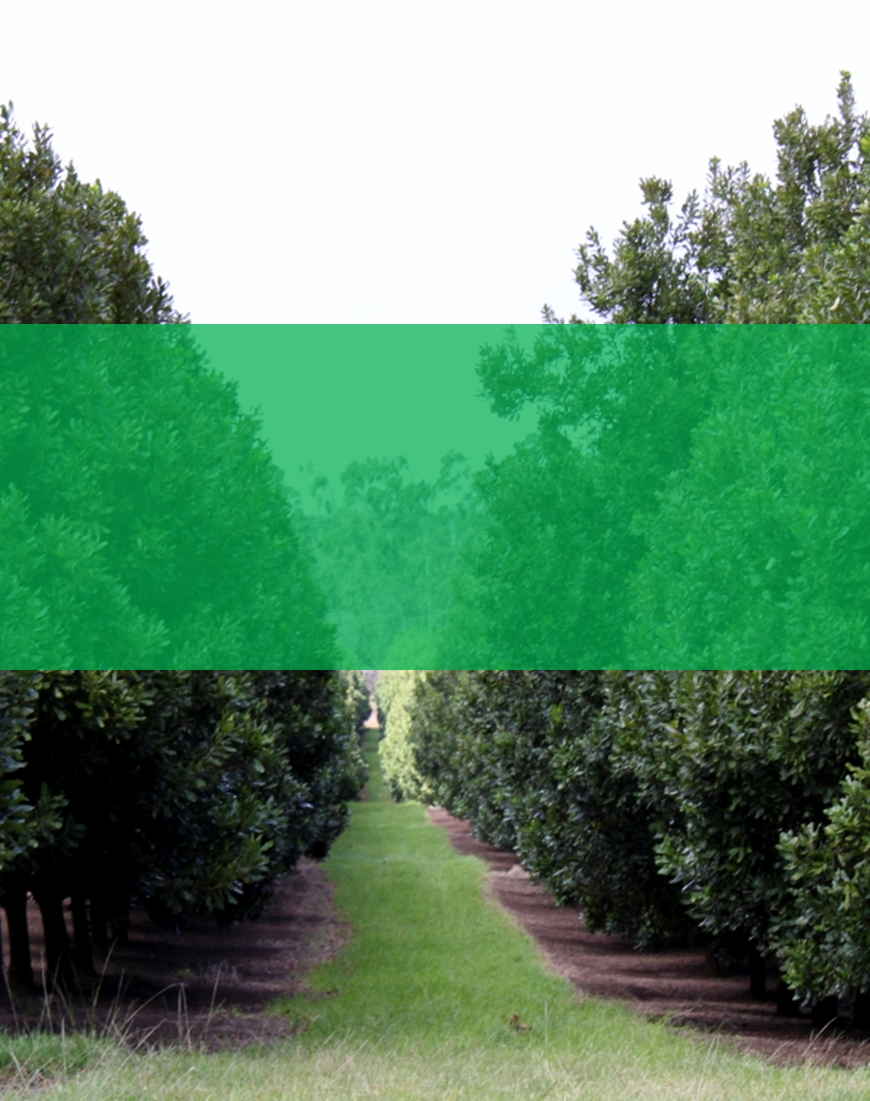
\includegraphics[scale=1]{frontcover}}} % Image background
\centering
\vspace*{5cm}
\par\normalfont\fontsize{35}{35}\sffamily\selectfont
\textbf{Harvest}\\
{\LARGE Functional Requirements and Application Design}\par % Book title
\vspace*{0.5cm}
{\Huge HTTP\_418}\par
\centering
\vspace*{0.5cm}
\begin{itemize}[label={}, noitemsep]	
		\Large
		\item \begin{center} Christiaan Saaiman, 12059138 \end{center}
		\item \begin{center} Michael Loosen, 14017254 \end{center}
		\item \begin{center} Elizabeth Bode, 14310156 \end{center}
		\item \begin{center} LC Meyers, 14024633 \end{center}	
\end{itemize}
\endgroup

%----------------------------------------------------------------------------------------
%	TABLE OF CONTENTS
%----------------------------------------------------------------------------------------

\chapterimage{orchard.png} % Table of contents heading image

\pagestyle{empty} % No headers

\tableofcontents % Print the table of contents itself

%\cleardoublepage % Forces the first chapter to start on an odd page so it's on the right

\pagestyle{fancy} % Print headers again

%----------------------------------------------------------------------------------------
%	CHAPTER 1
%----------------------------------------------------------------------------------------

\chapterimage{mangoes.png} % Chapter heading image

\chapter{Use Case Prioritization}
	\section{Critical}
	\begin{itemize}
		\item Login/Logout user
		\item Change Password
		\item Recover Password
		\item View/Edit/Create Farmer – Web interface
		\item View/Edit/Create Farm – Web interface
		\item View/Edit/Create Foreman – Web interface
		\item View/Edit/Create Worker – Web interface
		\item View/Create/Edit Orchard Block (crop dimensions, crop type, irrigation type, date planted, yields per hectare, cultivation frequency, yield measurement type) – Web interface
		\item View/Create/Edit Irrigation Type – Web interface
		\item View/Create/Edit Crop Type – Web interface
		\item View/Update Worker Performance (yields collected per worker)
		\item View/Create/Edit Yield Measurement Type (by farmer, eg. kg, bag, g, etc.) – Web interface
		\item View/Create/Edit Cultivation Frequency – Web interface
		\item Maintain Foreman-Orchard Block Allocations (allocate/deallocate foreman to orchard blocks) – Web interface
		\item View Foreman-Orchard Block Allocation – Web interface
		\item Maintain Worker-Foreman Assignments (assign/reassign workers to/from foreman) – Web interface
		\item View Worker-Foreman Assignment – Web interface
		
	\end{itemize}
	\section{Important}
	\begin{itemize}
		\item Import Census Data – Web interface
		\item Generate Statistical Report of Worker Performance (time intervals) – Web interface
		\item Generate Statistical Report Crop Yield per Orchard (potentially linked to heatmap generation) – Web interface				
	\end{itemize}
	\section{Nice-to-have}
	\begin{itemize}
		\item View Heat Map – Web interface
		\item View/Create/Edit Foreman’s Shift (potentially linked to location tracking)  – Web interface
		\item Notify Farmer Regarding Foreman’s Locations (according to time intervals)
		\item Notify Farmer of Foreman’s Activity History Every Half an Hour
		\item View/Delete Notifications
		\item Generate Revenue Report Regarding Seasonal Yields (to plan paying workers, operational costs, etc.) – Web interface
		\item Generate Statistical Report Regarding Time Taken to Yield Specific Crops– Web interface
	\end{itemize}
	


%----------------------------------------------------------------------------------------
%	CHAPTER 2
%----------------------------------------------------------------------------------------
\chapterimage{macadamias.png}
\chapter{Use Cases and Service Contracts}
\section{Login User}
\begin{itemize}
	\item Description\\
	This use case will be used by the users of the Web interface, Android interface and the iOS interface to initiate login via the back-end service.
	\item Pre-Conditions
	\begin{enumerate}
		\item The user has a registered account within the database.
		\item The user’s account is not locked.
	\end{enumerate}
	\item Post-Conditions
	\begin{enumerate}
		\item The user will be logged in and have access to the necessary functionality.
	\end{enumerate}
	\item Service Contract
	\begin{figure}
		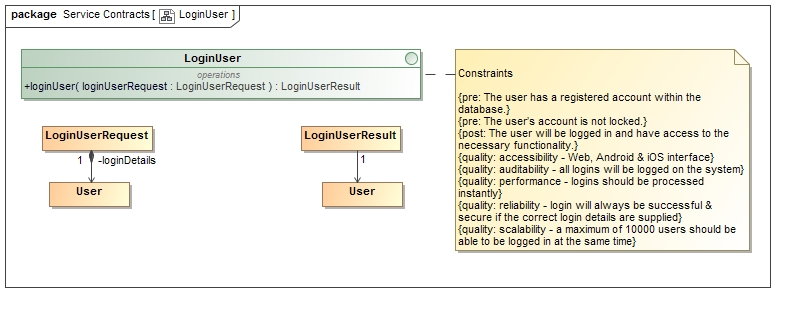
\includegraphics[scale=0.5]{ServiceContracts/class__LoginUser.jpg}
		\caption{Login User}
	\end{figure}
\end{itemize}

\section{Logout User}
\begin{itemize}
	\item Description\\
	This use case will be used by the users of the Web interface, Android interface and the iOS interface to log a user out of the system.
	\item Pre-Conditions
	\begin{enumerate}
		\item The user is currently logged into the system.
	\end{enumerate}
	\item Post-Conditions
	\begin{enumerate}
		\item The user will be logged out of the system and have no access to any functionality.
	\end{enumerate}
	\item Service Contract
	\begin{figure}
		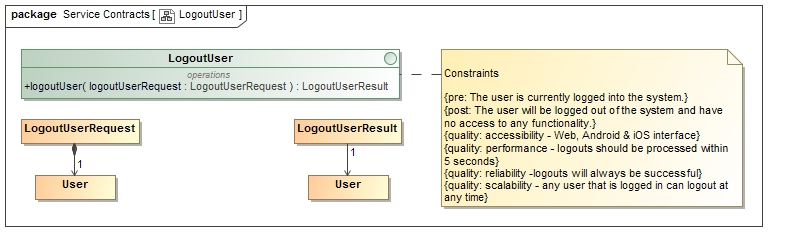
\includegraphics[scale=0.5]{ServiceContracts/class__LogoutUser.jpg}
		\caption{Logout User}
	\end{figure}
\end{itemize}

\section{Change Password}
\begin{itemize}
	\item Description\\
	This use case will be used by the users of the Web interface, Android interface and the iOS interface to change their password.
	\item Pre-Conditions
	\begin{enumerate}
		\item The user has a registered account within the database.
		\item The user’s account is not locked.
	\end{enumerate}
	\item Post-Conditions
	\begin{enumerate}
		\item The user’s password is updated in the database. 
	\end{enumerate}
	\item Service Contract
	\begin{figure}
		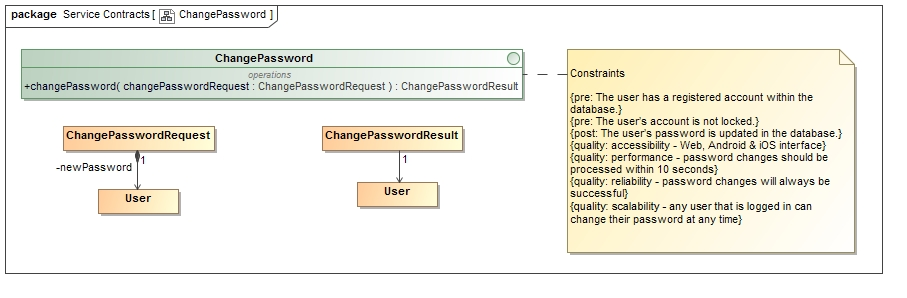
\includegraphics[scale=0.5]{ServiceContracts/class__ChangePassword.jpg}
		\caption{Change Password}
	\end{figure}
\end{itemize}

\section{Recover Password}
\begin{itemize}
	\item Description\\
	This use case will be used by the users of the Web interface, Android interface and the iOS interface to recover their forgotten password.
	\item Pre-Conditions
	\begin{enumerate}
		\item The user has a registered account within the database.
		\item The user’s account is not locked.
	\end{enumerate}
	\item Post-Conditions
	\begin{enumerate}
		\item The user will receive an email containing their password.
	\end{enumerate}
	\item Service Contract
	\begin{figure}
		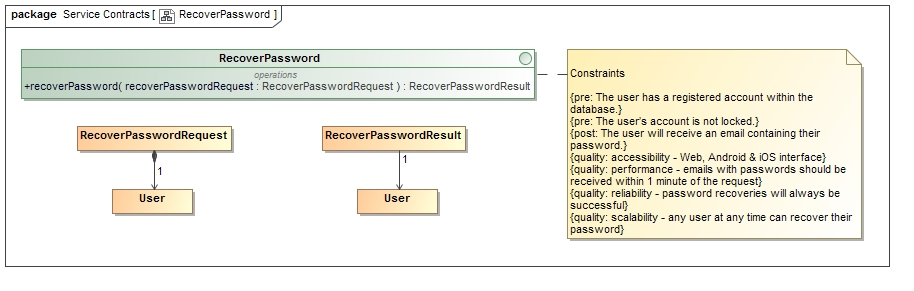
\includegraphics[scale=0.5]{ServiceContracts/class__RecoverPassword.jpg}
		\caption{Recover Password}
	\end{figure}
\end{itemize}

\section{Create Farmer}
\begin{itemize}
	\item Description\\
	This use case will be initiated by the farmer to create his superuser account for the system via the Web interface.
	\item Pre-Conditions
	\begin{enumerate}
		\item The farmer doesn’t already exist in the database.
	\end{enumerate}
	\item Post-Conditions
	\begin{enumerate}
		\item The farmer will have a superuser account registered in the database.
	\end{enumerate}
	\item Service Contract
	\begin{figure}
		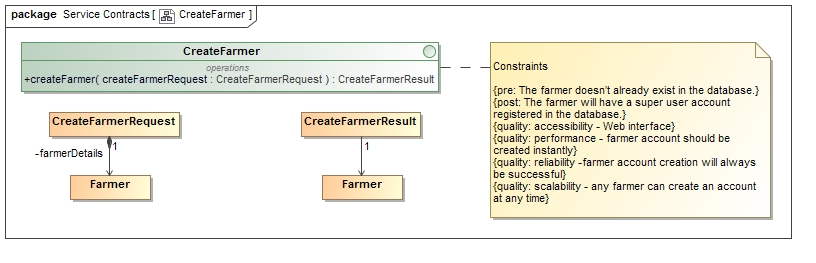
\includegraphics[scale=0.5]{ServiceContracts/class__CreateFarmer.jpg}
		\caption{Create Farmer}
	\end{figure}
\end{itemize}

\section{View Farmer}
\begin{itemize}
	\item Description\\
	This use case will be initiated by the farmer to view the current state of his superuser account for the system via the Web interface.
	\item Pre-Conditions
	\begin{enumerate}
		\item The farmer is currently logged into the system. (i.e. Super user logged in)
		\item The farmer already exists in the database.					
	\end{enumerate}
	\item Post-Conditions
	\begin{enumerate}
		\item The farmer’s account details will be displayed.
	\end{enumerate}
	\item Service Contract
	\begin{figure}
		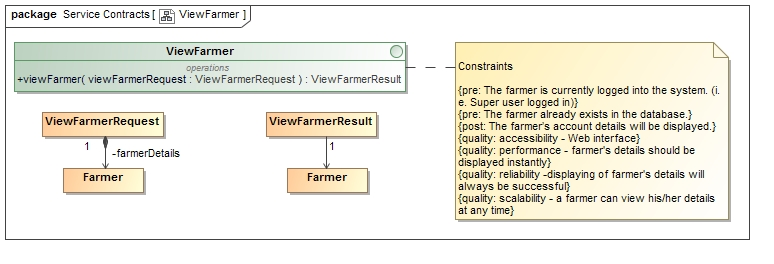
\includegraphics[scale=0.5]{ServiceContracts/class__ViewFarmer.jpg}
		\caption{View Farmer}
	\end{figure}
\end{itemize}

\section{Edit Farmer}
\begin{itemize}
	\item Description\\
	This use case will be initiated by the farmer to edit his superuser account for the system via the Web interface.
	\item Pre-Conditions
	\begin{enumerate}
		\item The farmer is currently logged into the system. (i.e. Super user logged in)
		\item The farmer already exists in the database.					
	\end{enumerate}
	\item Post-Conditions
	\begin{enumerate}
		\item The farmer’s details are updated in the database.
	\end{enumerate}
	\item Service Contract
	\begin{figure}
		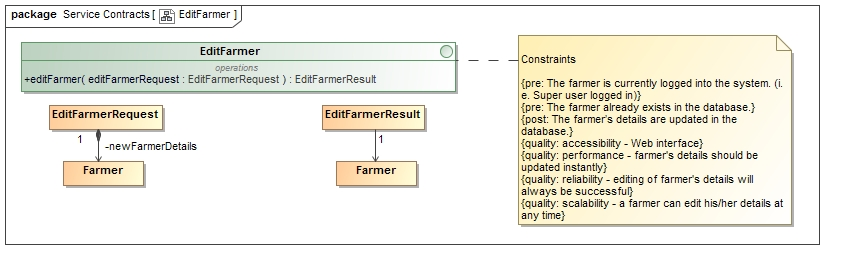
\includegraphics[scale=0.5]{ServiceContracts/class__EditFarmer.jpg}
		\caption{Edit Farmer}
	\end{figure}
\end{itemize}

\section{Create Farm}
\begin{itemize}
	\item Description\\
	This use case will be initiated by the farmer to register his farm on the system via the Web interface.
	\item Pre-Conditions
	\begin{enumerate}
		\item The farmer is currently logged into the system. (i.e. Super user logged in)
		\item The farm doesn’t already exist in the database.
	\end{enumerate}
	\item Post-Conditions
	\begin{enumerate}
		\item The farm is registered in the database.
	\end{enumerate}
	\item Service Contract
	\begin{figure}
		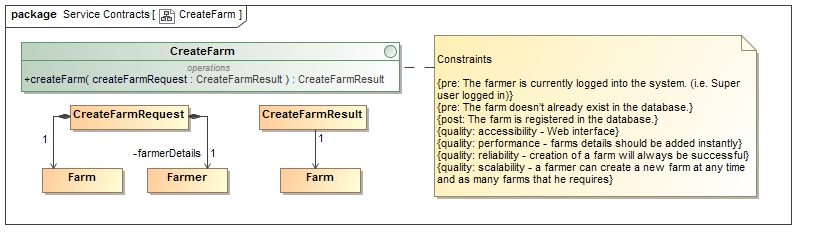
\includegraphics[scale=0.5]{ServiceContracts/class__CreateFarm.jpg}
		\caption{Create Farm}
	\end{figure}
\end{itemize}

\section{View Farm}
\begin{itemize}
	\item Description\\
	This use case will be initiated by the farmer to view the current state of his farm’s details on the system via the Web interface.
	\item Pre-Conditions
	\begin{enumerate}
		\item The farmer is currently logged into the system. (i.e. Super user logged in)
		\item The farm already exists in the database.					
	\end{enumerate}
	\item Post-Conditions
	\begin{enumerate}
		\item The farm’s account details will be displayed.
	\end{enumerate}
	\item Service Contract
	\begin{figure}
		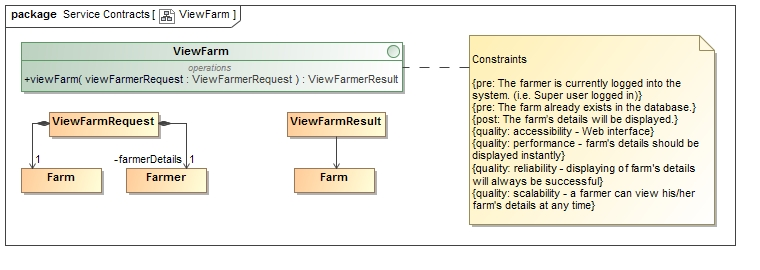
\includegraphics[scale=0.5]{ServiceContracts/class__ViewFarm.jpg}
		\caption{View Farm}
	\end{figure}
\end{itemize}

\section{Edit Farm}
\begin{itemize}
	\item Description\\
	This use case will be initiated by the farmer to edit his farm’s details on the system via the Web interface.
	\item Pre-Conditions
	\begin{enumerate}
		\item The farmer is currently logged into the system. (i.e. Super user logged in)
		\item The farm already exists in the database.					
	\end{enumerate}
	\item Post-Conditions
	\begin{enumerate}
		\item The farm’s details are updated in the database.
	\end{enumerate}
	\item Service Contract
	\begin{figure}
		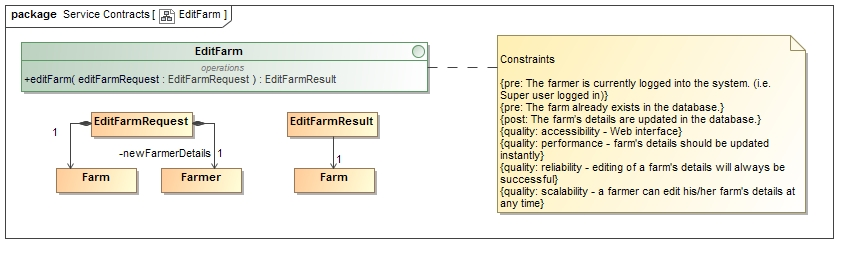
\includegraphics[scale=0.5]{ServiceContracts/class__EditFarm.jpg}
		\caption{Edit Farm}
	\end{figure}
\end{itemize}

%Foreman CRUD

%Worker CRUD

\section{Create Orchard Block}
\begin{itemize}
	\item Description\\
	This use case will be initiated by the farmer to create the orchard block on his farm according to map coordinates and by entering the necessary details (crop dimensions, crop type, irrigation type, date planted, yields per hectare) via the Web interface.
	\item Pre-Conditions
	\begin{enumerate}
		\item The farmer is currently logged into the system. (i.e. Super user logged in)
		\item The orchard block doesn't already exist.
	\end{enumerate}
	\item Post-Conditions
	\begin{enumerate}
		\item The new orchard block’s details are stored in the database.		
	\end{enumerate}
	\item Service Contract
	\begin{figure}
		\includegraphics[scale=0.5]{ServiceContracts/nameOfImage.png}
		\caption{Create Orchard Block}
	\end{figure}
\end{itemize}

\section{View Orchard Block}
\begin{itemize}
	\item Description\\
	This use case will be initiated by the farmer to view the orchard block on his farm via the Web interface.
	\item Pre-Conditions
	\begin{enumerate}
		\item The farmer is currently logged into the system. (i.e. Super user logged in)
		\item The orchard block already exists on the system.					
	\end{enumerate}
	\item Post-Conditions
	\begin{enumerate}
		\item The orchard block’s details are displayed.
	\end{enumerate}
	\item Service Contract
	\begin{figure}
		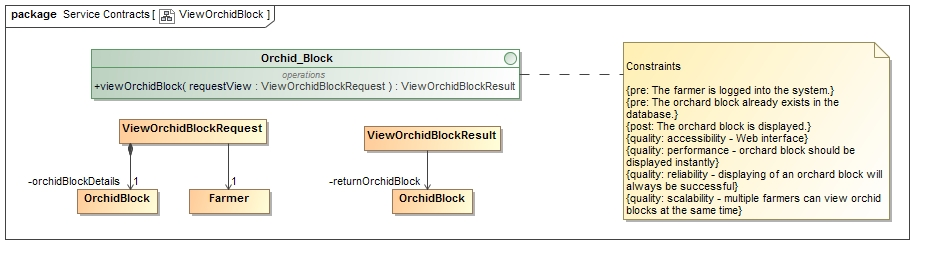
\includegraphics[scale=0.5]{ServiceContracts/class__ViewOrchidBlock.jpg}
		\caption{View Orchard Block}
	\end{figure}
\end{itemize}

\section{Edit Orchard Block (i.e. crop type, irrigation type, re-demarcate coordinates, archive, etc.)}
\begin{itemize}
	\item Description\\
	This use case will be initiated by the farmer to edit the orchard blocks on his farm via the Web interface.
	\item Pre-Conditions
	\begin{enumerate}
		\item The farmer is currently logged into the system. (i.e. Super user logged in)
		\item The orchard block already exists on the system.				
	\end{enumerate}
	\item Post-Conditions
	\begin{enumerate}
		\item The orchard block’s details are updated in the database.
	\end{enumerate}
	\item Service Contract
	\begin{figure}
		\includegraphics[scale=0.5]{ServiceContracts/nameOfImage.png}
		\caption{Edit Orchard Block}
	\end{figure}
\end{itemize}

\section{Create Irrigation Type}
\begin{itemize}
	\item Description\\
	This use case will be initiated by the farmer to create an irrigation type used on his farm on the system via the Web interface.
	\item Pre-Conditions
	\begin{enumerate}
		\item The farmer is currently logged into the system. (i.e. Super user logged in)
		\item The irrigation type doesn’t already exist in the database. 
	\end{enumerate}
	\item Post-Conditions
	\begin{enumerate}
		\item The irrigation type is added to the database.	
	\end{enumerate}
	\item Service Contract
	\begin{figure}
		\includegraphics[scale=0.5]{ServiceContracts/nameOfImage.png}
		\caption{Create Irrigation Type}
	\end{figure}
\end{itemize}

\section{View Irrigation Type}
\begin{itemize}
	\item Description\\
	This use case will be initiated by the farmer to view the current state of an irrigation type’s details on the system via the Web interface.
	\item Pre-Conditions
	\begin{enumerate}
		\item The farmer is currently logged into the system. (i.e. Super user logged in)
		\item The irrigation type already exists in the database.				
	\end{enumerate}
	\item Post-Conditions
	\begin{enumerate}
		\item The irrigation type’s details will be displayed.
	\end{enumerate}
	\item Service Contract
	\begin{figure}
		\includegraphics[scale=0.5]{ServiceContracts/nameOfImage.png}
		\caption{View Irrigation Type}
	\end{figure}
\end{itemize}

\section{Edit Irrigation Type}
\begin{itemize}
	\item Description\\
	This use case will be initiated by the farmer to edit an irrigation type’s details on the system via the Web interface.
	\item Pre-Conditions
	\begin{enumerate}
		\item The farmer is currently logged into the system. (i.e. Super user logged in)
		\item The irrigation type already exists in the database.					
	\end{enumerate}
	\item Post-Conditions
	\begin{enumerate}
		\item The irrigation type’s details are updated in the database.
	\end{enumerate}
	\item Service Contract
	\begin{figure}
		\includegraphics[scale=0.5]{ServiceContracts/nameOfImage.png}
		\caption{Edit Irrigation Type}
	\end{figure}
\end{itemize}

\section{Create Crop Type}
\begin{itemize}
	\item Description\\
	This use case will be initiated by the farmer to create a crop type planted on his farm on the system via the Web interface.
	\item Pre-Conditions
	\begin{enumerate}
		\item The farmer is currently logged into the system. (i.e. Super user logged in)
		\item The crop type doesn’t already exist in the database. 
	\end{enumerate}
	\item Post-Conditions
	\begin{enumerate}
		\item The crop type is added to the database.
	\end{enumerate}
	\item Service Contract
	\begin{figure}
		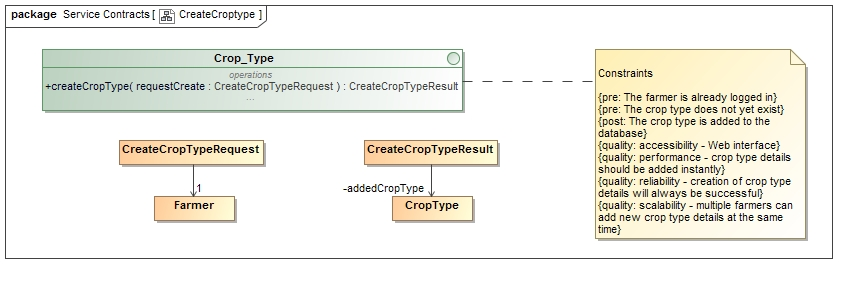
\includegraphics[scale=0.5]{ServiceContracts/class__CreateCroptype.jpg}
		\caption{Create Crop Type}
	\end{figure}
\end{itemize}

\section{View Crop Type}
\begin{itemize}
	\item Description\\
	This use case will be initiated by the farmer to view the current state of a crop type’s details on the system via the Web interface.
	\item Pre-Conditions
	\begin{enumerate}
		\item The farmer is currently logged into the system. (i.e. Super user logged in)
		\item The crop type already exists in the database.			
	\end{enumerate}
	\item Post-Conditions
	\begin{enumerate}
		\item The crop type’s details will be displayed.
	\end{enumerate}
	\item Service Contract
	\begin{figure}
		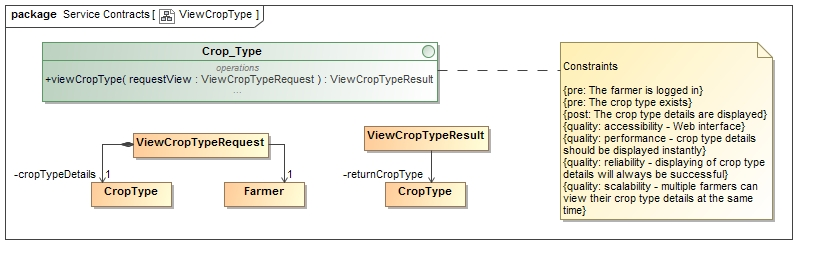
\includegraphics[scale=0.5]{ServiceContracts/class__ViewCropType.jpg}
		\caption{View Crop Type}
	\end{figure}
\end{itemize}

\section{Edit Crop Type}
\begin{itemize}
	\item Description\\
	This use case will be initiated by the farmer to edit a crop type’s details on the system via the Web interface.
	\item Pre-Conditions
	\begin{enumerate}
		\item The farmer is currently logged into the system. (i.e. Super user logged in)
		\item The crop type already exists in the database.					
	\end{enumerate}
	\item Post-Conditions
	\begin{enumerate}
		\item The crop type’s details are updated in the database
	\end{enumerate}
	\item Service Contract
	\begin{figure}
		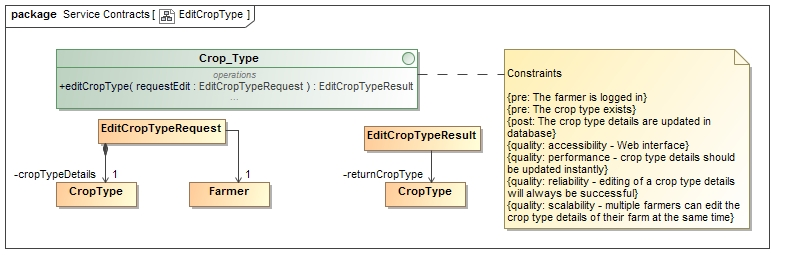
\includegraphics[scale=0.5]{ServiceContracts/class__EditCropType.jpg}
		\caption{Edit Crop Type}
	\end{figure}
\end{itemize}

%View and Update Worker Yield

\section{Create Yield Measurement Type}
\begin{itemize}
	\item Description\\
	This use case will be initiated by the farmer to create a yield measurement type used on his farm on the system via the Web interface.
	\item Pre-Conditions
	\begin{enumerate}
		\item The farmer is currently logged into the system. (i.e. Super user logged in)
		\item The yield measurement type doesn’t already exist in the database. 				
	\end{enumerate}
	\item Post-Conditions
	\begin{enumerate}
		\item The yield measurement type is added to the database.
	\end{enumerate}
	\item Service Contract
	\begin{figure}
		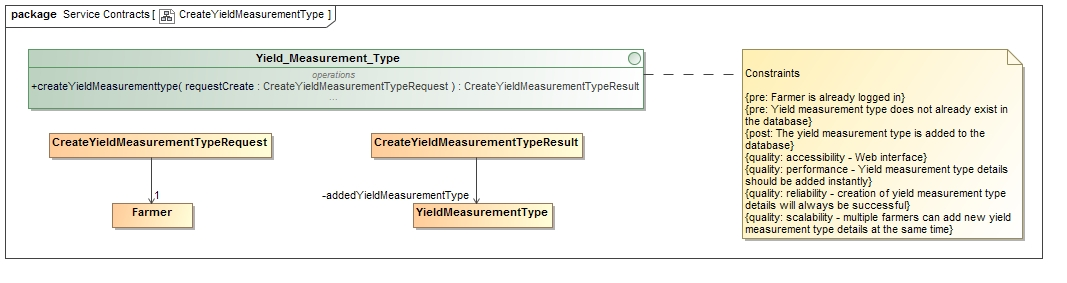
\includegraphics[scale=0.5]{ServiceContracts/class__CreateYieldMeasurementType.jpg}
		\caption{Create Yield Measurement Type}
	\end{figure}
\end{itemize}

\section{View Yield Measurement Type}
\begin{itemize}
	\item Description\\
	This use case will be initiated by the farmer to view the current state of a yield measurement type’s details on the system via the Web interface.
	\item Pre-Conditions
	\begin{enumerate}
		\item The farmer is currently logged into the system. (i.e. Super user logged in)
		\item The yield measurement type already exists in the database.		
	\end{enumerate}
	\item Post-Conditions
	\begin{enumerate}
		\item The yield measurement type’s details will be displayed.
	\end{enumerate}
	\item Service Contract
	\begin{figure}
		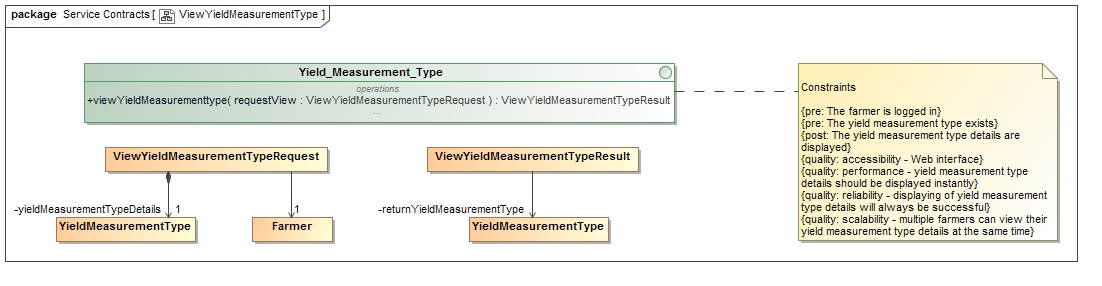
\includegraphics[scale=0.5]{ServiceContracts/class__ViewYieldMeasurementType.jpg}
		\caption{View Yield Measurement Type}
	\end{figure}
\end{itemize}

\section{Edit Yield Measurement Type}
\begin{itemize}
	\item Description\\
	This use case will be initiated by the farmer to edit a yield measurement type’s details on the system via the Web interface.
	\item Pre-Conditions
	\begin{enumerate}
		\item The farmer is currently logged into the system. (i.e. Super user logged in)
		\item The yield measurement type already exists in the database.					
	\end{enumerate}
	\item Post-Conditions
	\begin{enumerate}
		\item The yield measurement type’s details are updated in the database.
	\end{enumerate}
	\item Service Contract
	\begin{figure}
		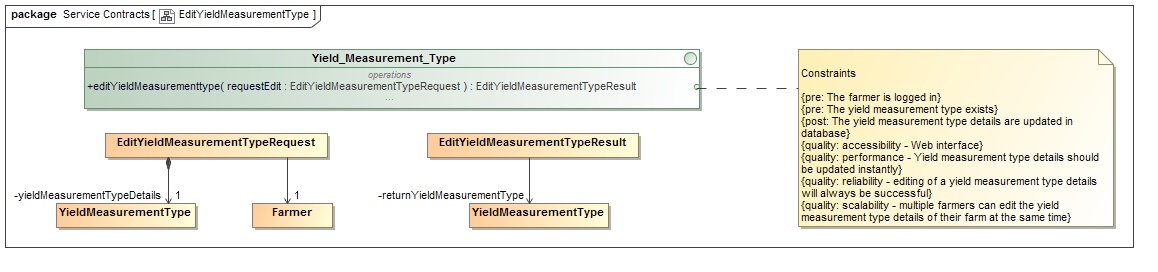
\includegraphics[scale=0.5]{ServiceContracts/class__EditYieldMeasurementType.jpg}
		\caption{Edit Yield Measurement Type}
	\end{figure}
\end{itemize}

\section{Create Cultivation Frequency}
\begin{itemize}
	\item Description\\
	This use case will be initiated by the farmer to create a cultivation frequency used on his farm on the system via the Web interface.
	\item Pre-Conditions
	\begin{enumerate}
		\item The farmer is currently logged into the system. (i.e. Super user logged in)
		\item The cultivation frequency doesn’t already exist in the database. 				
	\end{enumerate}
	\item Post-Conditions
	\begin{enumerate}
		\item The cultivation frequency is added to the database.
	\end{enumerate}
	\item Service Contract
	\begin{figure}
		\includegraphics[scale=0.5]{ServiceContracts/nameOfImage.png}
		\caption{Create Cultivation Frequency}
	\end{figure}
\end{itemize}

\section{View Cultivation Frequency}
\begin{itemize}
	\item Description\\
	This use case will be initiated by the farmer to view the current state of a cultivation frequency’s details on the system via the Web interface.
	\item Pre-Conditions
	\begin{enumerate}
		\item The farmer is currently logged into the system. (i.e. Super user logged in)
		\item The cultivation frequency already exists in the database.		
	\end{enumerate}
	\item Post-Conditions
	\begin{enumerate}
		\item The cultivation frequency’s details will be displayed.
	\end{enumerate}
	\item Service Contract
	\begin{figure}
		\includegraphics[scale=0.5]{ServiceContracts/nameOfImage.png}
		\caption{View Cultivation Frequency}
	\end{figure}
\end{itemize}

\section{Edit Cultivation Frequency}
\begin{itemize}
	\item Description\\
	This use case will be initiated by the farmer to edit a cultivation frequency’s details on the system via the Web interface.
	\item Pre-Conditions
	\begin{enumerate}
		\item The farmer is currently logged into the system. (i.e. Super user logged in)
		\item The cultivation frequency already exists in the database.					
	\end{enumerate}
	\item Post-Conditions
	\begin{enumerate}
		\item The cultivation frequency’s details are updated in the database.
	\end{enumerate}
	\item Service Contract
	\begin{figure}
		\includegraphics[scale=0.5]{ServiceContracts/nameOfImage.png}
		\caption{Edit Cultivation Frequency}
	\end{figure}
\end{itemize}

\section{Maintain Foreman-Orchard Block Allocations}
\begin{itemize}
	\item Description\\
	This use case will be initiated by the farmer to allocate or deallocate a specific foreman to/from a specific orchard block or multiple orchard blocks on his farm on the system via the Web interface.
	\item Pre-Conditions
	\begin{enumerate}
		\item The farmer is currently logged into the system. (i.e. Super user logged in)
		\item The foreman already exists in the database. 
		\item The orchard block already exists in the database.
		\item The foreman-orchard assignment already exists in the database. (For deallocation)					
	\end{enumerate}
	\item Post-Conditions
	\begin{enumerate}
		\item The foreman-orchard assignment is added to the database. (For allocation)
		\item The foreman-orchard assignment is removed from the database. (For deallocation)
	\end{enumerate}
	\item Service Contract
	\begin{figure}
		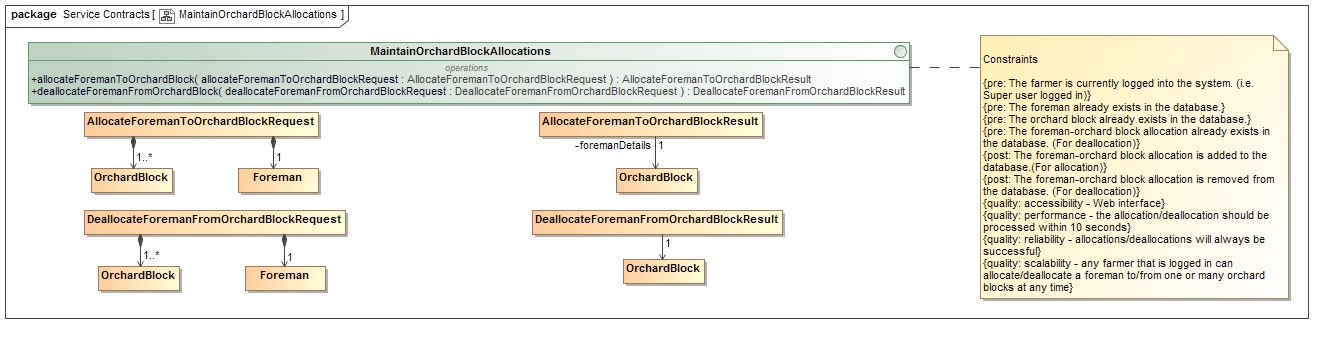
\includegraphics[scale=0.5]{ServiceContracts/class__MaintainOrchardBlockAllocations.jpg}
		\caption{Maintain Foreman-Orchard Block Allocations}
	\end{figure}
\end{itemize}

%Maintain Worker-Foreman Assingments

\section{Import Census Data}
\begin{itemize}
	\item Description\\
	This use case will be initiated by the farmer to import current census data onto the system via the Web interface to reduce the amount of data needed to be input manually.
	\item Pre-Conditions
	\begin{enumerate}
		\item The farmer is currently logged into the system. (i.e. Super user logged in)
		\item The census data is valid and in the correct format.								
	\end{enumerate}
	\item Post-Conditions
	\begin{enumerate}
		\item The census data is added and successfully integrated into the system.
	\end{enumerate}
	\item Service Contract
	\begin{figure}
		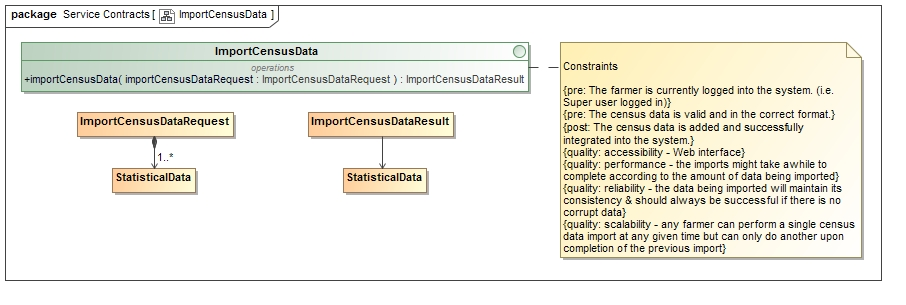
\includegraphics[scale=0.5]{ServiceContracts/class__ImportCensusData.jpg}
		\caption{Import Census Data}
	\end{figure}
\end{itemize}

\section{Generate Statistical Report of Worker Performance (according to time intervals)}
\begin{itemize}
	\item Description\\
	This use case will be initiated by the farmer to generate a report showing the performance of his workers during certain time intervals for statistical purposes via the Web interface.
	\item Pre-Conditions
	\begin{enumerate}
		\item The farmer is currently logged into the system. (i.e. Super user logged in)
		\item The data on the worker’s performance, required for the report, is present in the database.		
	\end{enumerate}
	\item Post-Conditions
	\begin{enumerate}
		\item The workers performance report has been generated in a usable format.
	\end{enumerate}
	\item Service Contract
	\begin{figure}
		\includegraphics[scale=0.5]{ServiceContracts/nameOfImage.png}
		\caption{Generate Statistical Report of Worker Performance (according to time intervals)}
	\end{figure}
\end{itemize}

\section{Generate Statistical Report of Crop Yield per Orchard}
\begin{itemize}
	\item Description\\
	This use case will be initiated by the farmer to generate a report showing the crop yield per orchard for statistical purposes via the Web interface.
	\item Pre-Conditions
	\begin{enumerate}
		\item The farmer is currently logged into the system. (i.e. Super user logged in)
		\item The data on the crop yields for each orchard, required for the report, is present in the database.									
	\end{enumerate}
	\item Post-Conditions
	\begin{enumerate}
		\item The crop yield per orchard report has been generated in a usable format.
	\end{enumerate}
	\item Service Contract
	\begin{figure}
		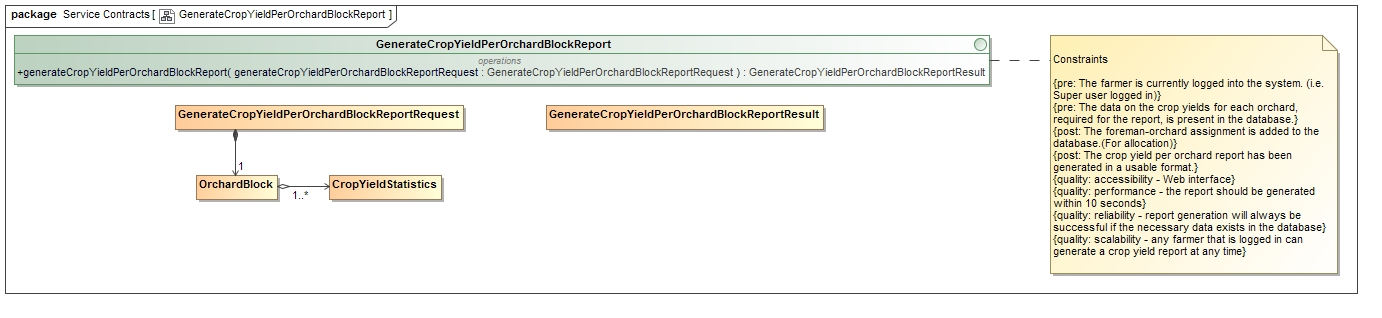
\includegraphics[scale=0.5]{ServiceContracts/class__GenerateCropYieldPerOrchardBlockReport.jpg}
		\caption{Generate Statistical Report of Crop Yield per Orchard}
	\end{figure}
\end{itemize}

\section{View Heat Map}
\begin{itemize}
	\item Description\\
	This use case will be initiated by the farmer to view the crop yields per orchard blocks according to a heat map via the Web interface.
	\item Pre-Conditions
	\begin{enumerate}
		\item The farmer is currently logged into the system. (i.e. Super user logged in)
		\item The data on the crop yields for each orchard, required to generate the heat map, is present in the database.	
	\end{enumerate}
	\item Post-Conditions
	\begin{enumerate}
		\item The crop yield per orchard heat map is generated and displayed.
	\end{enumerate}
	\item Service Contract
	\begin{figure}
		\includegraphics[scale=0.5]{ServiceContracts/nameOfImage.png}
		\caption{View Heat Map}
	\end{figure}
\end{itemize}

\section{Create Foreman’s Shift}
\begin{itemize}
	\item Description\\
	This use case will be initiated by the farmer to allocate a foreman to a specific shift on the system via the Web interface.
	\item Pre-Conditions
	\begin{enumerate}
		\item The farmer is currently logged into the system. (i.e. Super user logged in)
		\item The foreman already exists in the database. 
		\item The foreman-shift assignment doesn’t exist in the database.					
	\end{enumerate}
	\item Post-Conditions
	\begin{enumerate}
		\item The foreman-shift assignment is added to the database.
	\end{enumerate}
	\item Service Contract
	\begin{figure}
		\includegraphics[scale=0.5]{ServiceContracts/nameOfImage.png}
		\caption{Create Foreman’s Shift}
	\end{figure}
\end{itemize}

\section{View Foreman’s Shift}
\begin{itemize}
	\item Description\\
	This use case will be initiated by the farmer to view the current state of a foreman’s shift details on the system via the Web interface.
	\item Pre-Conditions
	\begin{enumerate}
		\item The farmer is currently logged into the system. (i.e. Super user logged in)
		\item The foreman-shift assignment already exists in the database.		
	\end{enumerate}
	\item Post-Conditions
	\begin{enumerate}
		\item The foreman-shift assignment details will be displayed.
	\end{enumerate}
	\item Service Contract
		\begin{figure}
			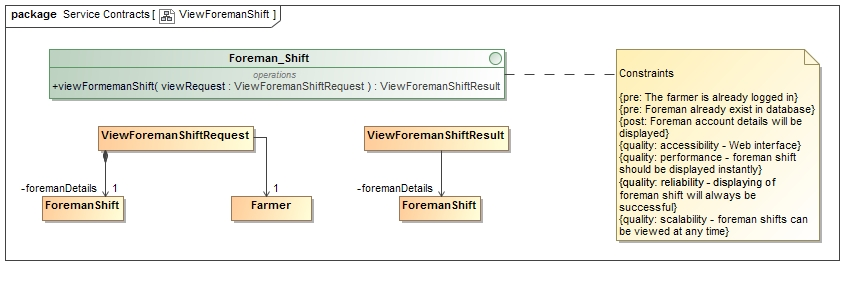
\includegraphics[scale=0.5]{ServiceContracts/class__ViewForemanShift.jpg}
			\caption{View Foreman’s Shift}
		\end{figure}
\end{itemize}

\section{Edit Foreman’s Shift}
\begin{itemize}
	\item Description\\
	This use case will be initiated by the farmer to edit a foreman’s shift details on the system via the Web interface.
	\item Pre-Conditions
	\begin{enumerate}
		\item The farmer is currently logged into the system. (i.e. Super user logged in)
		\item The foreman-shift assignment already exists in the database.	
	\end{enumerate}
	\item Post-Conditions
	\begin{enumerate}
		\item The foreman-shift assignment details are updated in the database.
	\end{enumerate}
	\item Service Contract
	\begin{figure}
		\includegraphics[scale=0.5]{ServiceContracts/nameOfImage.png}
		\caption{Edit Foreman’s Shift}
	\end{figure}
\end{itemize}

\section{Notify Farmer Regarding Foreman’s Locations (according to time intervals)}
\begin{itemize}
	\item Description\\
	This use case will be initiated when a foreman leaves the demarcated area he has been allocated during his shift hours. When this occurs, a SMS or in-app notification will alert the farmer regarding this unusual occurrence via the Android or iOS interface.
	\item Pre-Conditions
	\begin{enumerate}
		\item The farmer is currently logged into the system on his mobile device. (i.e. Super user logged in)
		\item The foreman is logged into the system on his mobile device.
		\item The data regarding the foreman’s shift, allocated orchard block and his current GPS location are available to initiate the notification.						
	\end{enumerate}
	\item Post-Conditions
	\begin{enumerate}
		\item The farmer receives an SMS or an in-app notification regarding the foreman’s current location.
	\end{enumerate}
	\item Service Contract
	\begin{figure}
		\includegraphics[scale=0.5]{ServiceContracts/nameOfImage.png}
		\caption{Notify Farmer Regarding Foreman’s Locations}
	\end{figure}
\end{itemize}

\section{Notify Farmer of Foreman’s Activity History Every Half an Hour}
\begin{itemize}
	\item Description\\
	This use case will be initiated every half an hour to notify the farmer on his moble device regarding the foreman’s activity history to prevent theft.
	\item Pre-Conditions
	\begin{enumerate}
		\item The farmer is currently logged into the system on his mobile device. (i.e. Super user logged in)
		\item The foreman is logged into the system on his mobile device.
		\item The foreman’s activity history is present in the database.					
	\end{enumerate}
	\item Post-Conditions
	\begin{enumerate}
		\item The farmer receives an SMS or an in-app notification every half an hour regarding the foreman’s activity history.
	\end{enumerate}
	\item Service Contract
	\begin{figure}
		\includegraphics[scale=0.5]{ServiceContracts/nameOfImage.png}
		\caption{Notify Farmer of Foreman’s Activity History Every Half an Hour}
		\end{figure}
\end{itemize}

\section{Generate Revenue Report Regarding Seasonal Yields}
\begin{itemize}
	\item Description\\
	This use case will be initiated by the farmer to generate a report showing the revenue generated according to seasonal yields per orchard block for statistical purposes via the Web interface.
	\item Pre-Conditions
	\begin{enumerate}
		\item The farmer is currently logged into the system. (i.e. Super user logged in)
		\item The data on the crop yields for each orchard and the related revenue, required for the report, is present in the database.	
	\end{enumerate}
	\item Post-Conditions
	\begin{enumerate}
		\item The revenue per orchard report has been generated in a usable format.
	\end{enumerate}
	\item Service Contract
	\begin{figure}
		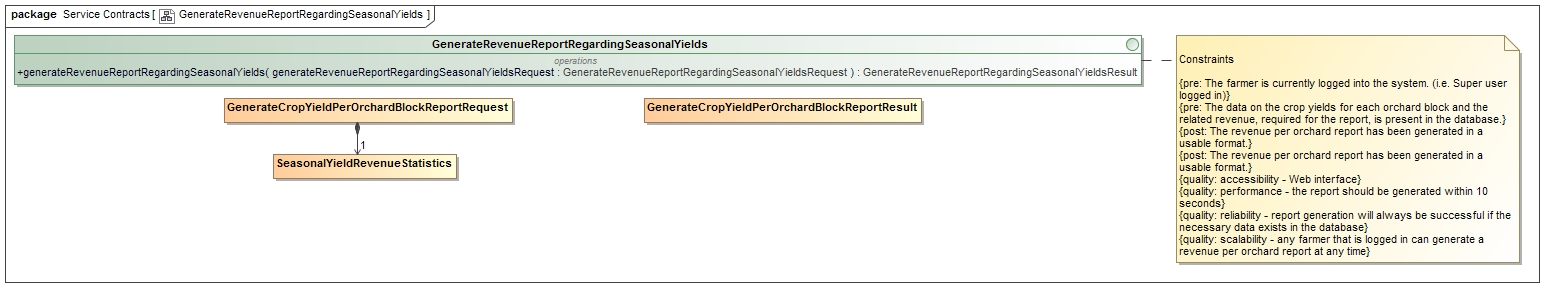
\includegraphics[scale=0.5]{ServiceContracts/class__GenerateRevenueReportRegardingSeasonalYields.jpg}
		\caption{Generate Revenue Report Regarding Seasonal Yields}
	\end{figure}
\end{itemize}

%Generate Report



%----------------------------------------------------------------------------------------
%	CHAPTER 3
%----------------------------------------------------------------------------------------

\chapterimage{avocados.png}
\chapter{Use Case Functionality} % Use case diagrams

	\section{Login User}
	\begin{figure}
		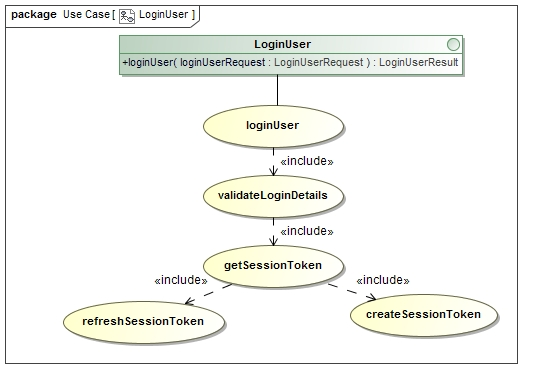
\includegraphics[scale=0.5]{UseCaseDiagrams/uc__LoginUser.jpg}
		\caption{Login User}
	\end{figure}
	
	\section{Logout User}
	\begin{figure}
		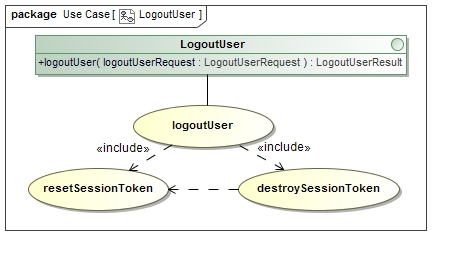
\includegraphics[scale=0.5]{UseCaseDiagrams/uc__LogoutUser.jpg}
		\caption{Logout User}
	\end{figure}
	
	\section{Change Password}
	\begin{figure}
		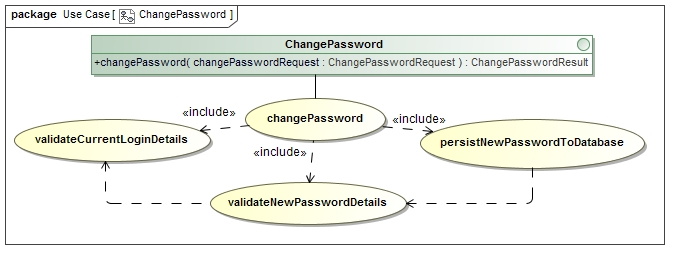
\includegraphics[scale=0.5]{UseCaseDiagrams/uc__ChangePassword.jpg}
		\caption{Change Password}
	\end{figure}
	
	\section{Recover Password}
	\begin{figure}
		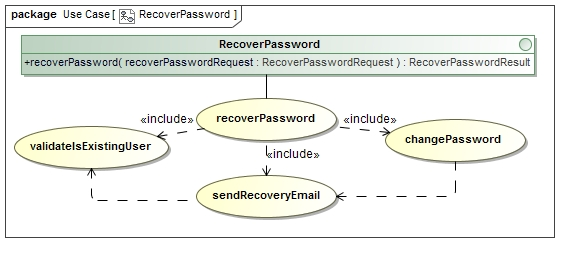
\includegraphics[scale=0.5]{UseCaseDiagrams/uc__RecoverPassword.jpg}
		\caption{Recover Password}
	\end{figure}
	
	
	\section{Create Farmer}
	\begin{figure}
		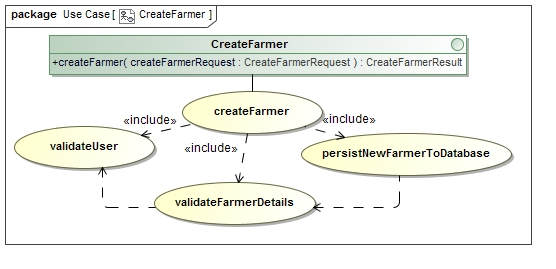
\includegraphics[scale=0.5]{UseCaseDiagrams/uc__CreateFarmer.jpg}
		\caption{Create Farmer}
	\end{figure}
	
	\section{View Farmer}
	\begin{figure}
		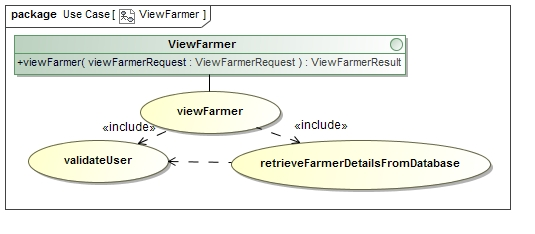
\includegraphics[scale=0.5]{UseCaseDiagrams/uc__ViewFarmer.jpg}
		\caption{View Farmer}
	\end{figure}
	
	\section{Edit Farmer}
	\begin{figure}
		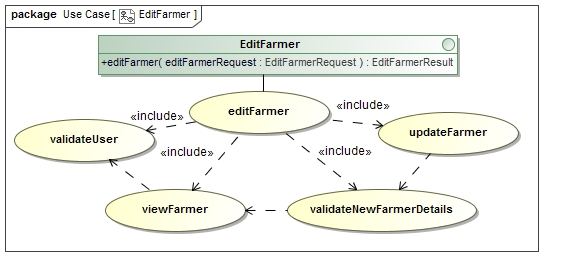
\includegraphics[scale=0.5]{UseCaseDiagrams/uc__EditFarmer.jpg}
		\caption{Edit Farmer}
	\end{figure}
	
	\section{Create Farm}
	\begin{figure}
		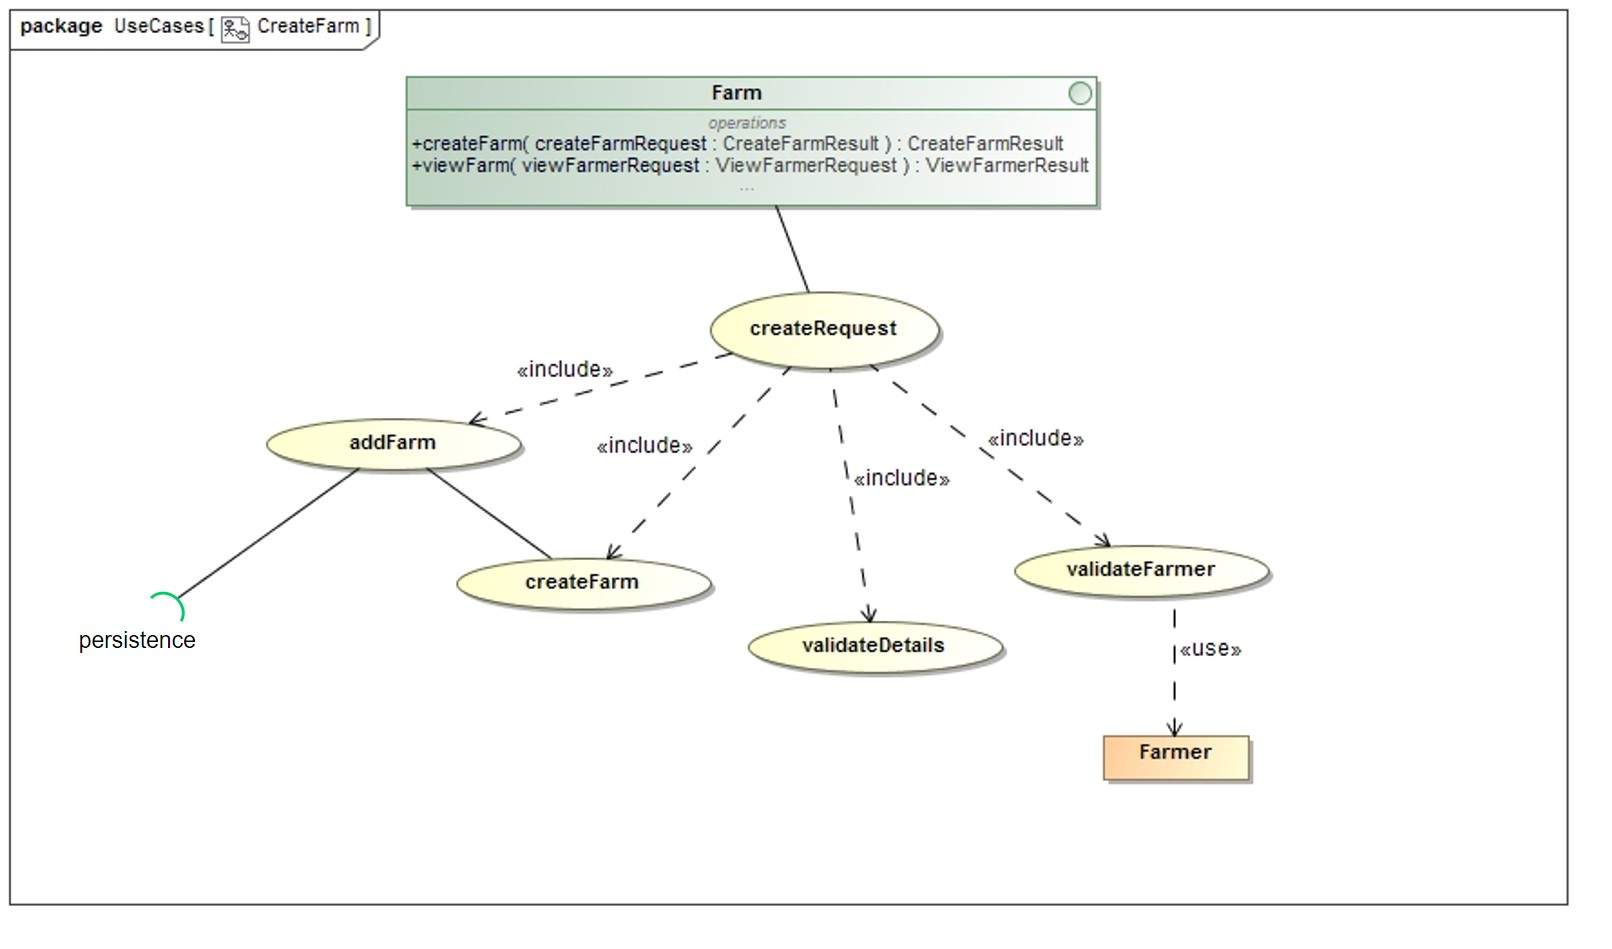
\includegraphics[scale=0.5]{UseCaseDiagrams/uc__CreateFarm.jpg}
		\caption{Create Farm}
	\end{figure}
	
	\section{View Farm}
	\begin{figure}
		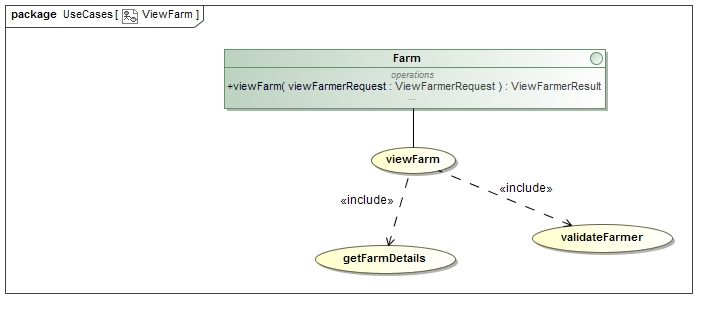
\includegraphics[scale=0.5]{UseCaseDiagrams/uc__ViewFarm.jpg}
		\caption{View Farm}
	\end{figure}
	
	\section{Edit Farm}
	\begin{figure}
		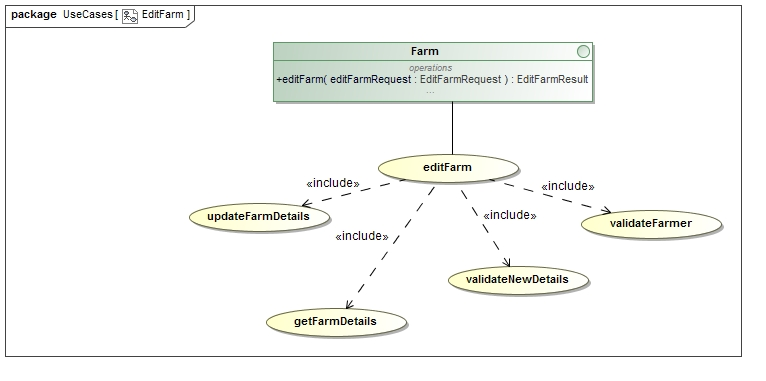
\includegraphics[scale=0.5]{UseCaseDiagrams/uc__EditFarm.jpg}
		\caption{Edit Farm}
	\end{figure}
	
	
	\section{Create Foreman}
	\begin{figure}
		\includegraphics[scale=0.5]{UseCaseDiagrams/nameOfImage.png}
		\caption{Create Foreman}
	\end{figure}
	
	\section{View Foreman}
	\begin{figure}
		\includegraphics[scale=0.5]{UseCaseDiagrams/nameOfImage.png}
		\caption{View Foreman}
	\end{figure}
	
	\section{Edit Foreman}
	\begin{figure}
		\includegraphics[scale=0.5]{UseCaseDiagrams/nameOfImage.png}
		\caption{Edit Foreman}
	\end{figure}
	
	\section{Create Worker}
	\begin{figure}
		\includegraphics[scale=0.5]{UseCaseDiagrams/nameOfImage.png}
		\caption{Create Worker}
	\end{figure}
	
	\section{View Worker}
	\begin{figure}
		\includegraphics[scale=0.5]{UseCaseDiagrams/nameOfImage.png}
		\caption{View Worker}
	\end{figure}
	
	\section{Edit Worker}
	\begin{figure}
		\includegraphics[scale=0.5]{UseCaseDiagrams/nameOfImage.png}
		\caption{Edit Worker}
	\end{figure}
	
	\section{Create Orchard Block}
	\begin{figure}
		\includegraphics[scale=0.5]{UseCaseDiagrams/nameOfImage.png}
		\caption{Create Orchard Block}
	\end{figure}
	
	\section{View Orchard Block}
	\begin{figure}
		\includegraphics[scale=0.5]{UseCaseDiagrams/uc__ViewOrchidBlock.jpg}
		\caption{View Orchard Block}
	\end{figure}
	
	\clearpage
	\section{Edit Orchard Block (i.e. crop type, irrigation type, re-demarcate coordinates, archive, etc.)}
	\begin{figure}
		\includegraphics[scale=0.5]{UseCaseDiagrams/nameOfImage.png}
		\caption{Edit Orchard Block}
	\end{figure}
	
	
	\section{Create Irrigation Type}
	\begin{figure}
		\includegraphics[scale=0.5]{UseCaseDiagrams/nameOfImage.png}
		\caption{Create Irrigation Type}
	\end{figure}
	
	\section{View Irrigation Type}
	\begin{figure}
		\includegraphics[scale=0.5]{UseCaseDiagrams/nameOfImage.png}
		\caption{View Irrigation Type}
	\end{figure}
	
	\section{Edit Irrigation Type}
	\begin{figure}
		\includegraphics[scale=0.5]{UseCaseDiagrams/nameOfImage.png}
		\caption{Edit Irrigation Type}
	\end{figure}
	
	
	\section{Create Crop Type}
	\begin{figure}
		\includegraphics[scale=0.5]{UseCaseDiagrams/uc__CreateCropType.jpg}
		\caption{Create Crop Type}
	\end{figure}
	
	\section{View Crop Type}
	\begin{figure}
		\includegraphics[scale=0.5]{UseCaseDiagrams/uc__ViewCropType.jpg}
		\caption{View Crop Type}
	\end{figure}
	
	\section{Edit Crop Type}
	\begin{figure}
		\includegraphics[scale=0.5]{UseCaseDiagrams/uc__EditCroptype.jpg}
		\caption{Edit Crop Type}
	\end{figure}
	
	\section{View Worker Performance}
	\begin{figure}
		\includegraphics[scale=0.5]{UseCaseDiagrams/nameOfImage.png}
		\caption{View Worker Performance}
	\end{figure}
	
	\section{Update Worker Performance}
	\begin{figure}
		\includegraphics[scale=0.5]{UseCaseDiagrams/nameOfImage.png}
		\caption{Update Worker Performance}
	\end{figure}
	
	\section{Create Yield Measurement Type}
	\begin{figure}
		\includegraphics[scale=0.5]{UseCaseDiagrams/uc__CreateYieldMeasurementType.jpg}
		\caption{Create Yield Measurement Type}
	\end{figure}
	
	\section{View Yield Measurement Type}
	\begin{figure}
		\includegraphics[scale=0.5]{UseCaseDiagrams/uc__ViewYieldMeasurementType.jpg}
		\caption{View Yield Measurement Type}
	\end{figure}
	
	\section{Edit Yield Measurement Type}
	\begin{figure}
		\includegraphics[scale=0.5]{UseCaseDiagrams/uc__EditYieldMeasurementType.jpg}
		\caption{Edit Yield Measurement Type}
	\end{figure}
	
	\section{Create Cultivation Frequency}
	\begin{figure}
		\includegraphics[scale=0.5]{UseCaseDiagrams/nameOfImage.png}
		\caption{Create Cultivation Frequency}
	\end{figure}
	
	\section{View Cultivation Frequency}
	\begin{figure}
		\includegraphics[scale=0.5]{UseCaseDiagrams/nameOfImage.png}
		\caption{View Cultivation Frequency}
	\end{figure}
	
	\section{Edit Cultivation Frequency}
	\begin{figure}
		\includegraphics[scale=0.5]{UseCaseDiagrams/nameOfImage.png}
		\caption{Edit Cultivation Frequency}
	\end{figure}
	
	
	\section{Maintain Foreman-Orchard Block Allocations}
	\begin{figure}
		\includegraphics[scale=0.5]{UseCaseDiagrams/uc__MaintainForemanOrchardBlockAllocations.jpg}
		\caption{Maintain Foreman-Orchard Block Allocations}
	\end{figure}
	
	\section{Maintain Worker-Foreman Assignments}
	\begin{figure}
		\includegraphics[scale=0.5]{UseCaseDiagrams/uc__ViewWorkerForemanAssignment.jpg}
		\caption{Maintain Worker-Foreman Assignments}
	\end{figure}
	
	\section{Import Census Data}
	\begin{figure}
		\includegraphics[scale=0.5]{UseCaseDiagrams/uc__ImportCensusData.jpg}
		\caption{Import Census Data}
	\end{figure}
	
	\section{Generate Statistical Report of Worker Performance (according to time intervals)}
	\begin{figure}
		\includegraphics[scale=0.5]{UseCaseDiagrams/nameOfImage.png}
		\caption{Generate Statistical Report of Worker Performance (according to time intervals)}
	\end{figure}
	
	\section{Generate Statistical Report of Crop Yield per Orchard}
	\begin{figure}
		\includegraphics[scale=0.5]{UseCaseDiagrams/uc__GenerateCropYieldPerOrchardBlockReport.jpg}
		\caption{Generate Statistical Report of Crop Yield per Orchard}
	\end{figure}
	
	\section{View Heat Map}
	\begin{figure}
		\includegraphics[scale=0.5]{UseCaseDiagrams/nameOfImage.png}
		\caption{View Heat Map}
	\end{figure}
	
	\section{Create Foreman’s Shift}
	\begin{figure}
		\includegraphics[scale=0.5]{UseCaseDiagrams/nameOfImage.png}
		\caption{Create Foreman’s Shift}
	\end{figure}
	
	\section{View Foreman’s Shift}
	\begin{figure}
		\includegraphics[scale=0.5]{UseCaseDiagrams/uc__ViewForemanShift.jpg}
		\caption{View Foreman’s Shift}
	\end{figure}
	
	\section{Edit Foreman’s Shift}
	\begin{figure}
		\includegraphics[scale=0.5]{UseCaseDiagrams/nameOfImage.png}
		\caption{Edit Foreman’s Shift}
	\end{figure}
	
	\section{Notify Farmer Regarding Foreman’s Locations (according to time intervals)}
	\begin{figure}
		\includegraphics[scale=0.5]{UseCaseDiagrams/nameOfImage.png}
		\caption{Notify Farmer Regarding Foreman’s Locations}
	\end{figure}
	
	\section{Notify Farmer of Foreman’s Activity History Every Half an Hour}
	\begin{figure}
		\includegraphics[scale=0.5]{UseCaseDiagrams/nameOfImage.png}
		\caption{Notify Farmer of Foreman’s Activity History Every Half an Hour}
	\end{figure}
	
	\section{Generate Revenue Report Regarding Seasonal Yields}
	\begin{figure}
		\includegraphics[scale=0.5]{UseCaseDiagrams/uc__GenerateRevenueReportRegardingSeasonalYields.jpg}
		\caption{Generate Revenue Report Regarding Seasonal Yields}
	\end{figure}
	
	\section{Generate Statistical Report Regarding Time Taken to Yield Specific Crops}
	\begin{figure}
		\includegraphics[scale=0.5]{UseCaseDiagrams/nameOfImage.png}
		\caption{Generate Statistical Report Regarding Time Taken to Yield Specific Crops}
	\end{figure}


%----------------------------------------------------------------------------------------
%	CHAPTER 4
%----------------------------------------------------------------------------------------

\chapterimage{litchis.png} % Chapter heading image

\chapter{Use Case Process Specifications} % Activity diagrams

\section{Login User}
\begin{figure}
	\includegraphics[scale=0.5]{ActivityDiagrams/act__Activity_Diagrams__LoginUser.jpg}
	\caption{Login User}
\end{figure}

\section{Logout User}
\begin{figure}
	\includegraphics[scale=0.5]{ActivityDiagrams/nameOfImage.png}
	\caption{Logout User}
\end{figure}

\section{Change Password}
\begin{figure}
	\includegraphics[scale=0.5]{ActivityDiagrams/act__Activity_Diagrams__ChangePassword.jpg}
	\caption{Change Password}
\end{figure}

\section{Recover Password}
\begin{figure}
	\includegraphics[scale=0.5]{ActivityDiagrams/act__Activity_Diagrams__RecoverPassword.jpg}
	\caption{Recover Password}
\end{figure}

\section{Allocate Foreman To Orchard Block}
\begin{figure}
	\includegraphics[scale=0.5]{ActivityDiagrams/act__Activity_Diagrams__AllocateForemanToOrchardBlock.jpg}
	\caption{Allocate Foreman To Orchard Block}
\end{figure}

\section{Deallocate Foreman From Orchard Block}
\begin{figure}
	\includegraphics[scale=0.5]{ActivityDiagrams/act__Activity_Diagrams__DeallocateForemanFromOrchardBlock.jpg}
	\caption{Deallocate Foreman From Orchard Block}
\end{figure}

\section{Import Census Data}
\begin{figure}
	\includegraphics[scale=0.5]{ActivityDiagrams/act__Activity_Diagrams__ImportCensusData.jpg}
	\caption{Import Census Data}
\end{figure}

\section{Generate Statistical Report of Worker Performance (according to time intervals)}
\begin{figure}
	\includegraphics[scale=0.5]{ActivityDiagrams/nameOfImage.png}
	\caption{Generate Statistical Report of Worker Performance (according to time intervals)}
\end{figure}

%----------------------------------------------------------------------------------------
%	CHAPTER 5
%----------------------------------------------------------------------------------------

\chapterimage{litchiTree.png} % Chapter heading image

\chapter{Domain Model}

\begin{figure}
	\includegraphics[scale=0.5]{nameOfImage}
	\caption{Domain Model}
\end{figure}
	
	
%----------------------------------------------------------------------------------------
%	CHAPTER 6
%----------------------------------------------------------------------------------------

\chapterimage{farmer.png} % Chapter heading image

\chapter{Open Issues}

\section{Database Issues}
\begin{itemize}
	\item We are not exactly sure how we are going to design our database and store data. We do not yet know if we need relationships or not
	\item We have not yet decided on a proper local database that takes advantage of HTML5 Local Storage.
\end{itemize}

\end{document}